\documentclass[twoside,11pt,b5paper,twocolumn]{scrbook}
\usepackage{fontspec} % To use a beautiful font
\defaultfontfeatures{RawFeature={+hlig,+clig,+dlig,+cv11,+cv90,+calt,+ccmp,+swsh},%
  Numbers={Proportional,OldStyle},%
  SmallCapsFeatures={RawFeature={+smcp}},}


\usepackage[hidelinks]{hyperref} % check and put cross-references
\usepackage[british]{babel} % hyphenation
\usepackage{xcolor} % have colors
\definecolor{marron}{RGB}{60,30,10}
\definecolor{darkblue}{RGB}{0,0,80}
\definecolor{lightblue}{RGB}{80,80,80}
\definecolor{darkgreen}{RGB}{0,80,0}
\definecolor{lightgreen}{RGB}{10,100,20}
\definecolor{darkgray}{RGB}{0,80,0}
\definecolor{darkred}{RGB}{80,0,0}
\definecolor{shadecolor}{rgb}{0.97,0.97,0.97}

\usepackage{wrapfig}
\usepackage{booktabs}
\usepackage{tabularx}
\usepackage{graphicx}
\usepackage{scrlayer-scrpage} % have fancy headers and footers
\usepackage{lettrine} % For dopped capitals
\usepackage{dblfloatfix} % for specifying two-column table placement
\usepackage{fixltx2e} % for fixing two-column table placement
\usepackage[tmargin=2cm, bmargin=3cm,
lmargin=3cm, rmargin=1.5cm,
headheight=1.0cm,
headsep=0.4cm, footskip=1.5cm]{geometry}


\usepackage[final,stretch=10,protrusion=true,expansion=true]{microtype}
\microtypecontext{spacing=nonfrench}

\setmainfont[SmallCapsFont={EB Garamond}]{EB Garamond}
\setkomafont{disposition}{\rmfamily}

\setlength{\parskip}{1.3ex plus 0.2ex minus 0.2ex}


\usepackage{fourier-orns}

\newcommand{\ornamento}{\vspace{2em}\noindent \textcolor{darkgray}{\hrulefill~ \raisebox{-2.5pt}[10pt][10pt]{\leafright \decofourleft \decothreeleft \aldineright \decotwo \floweroneleft \decoone \floweroneright \decotwo \aldineleft\decothreeright \decofourright \leafleft} ~ \hrulefill \\ \vspace{2em}}}
\newcommand{\ornpar}{\noindent \textcolor{darkgray}{ \raisebox{-1.9pt}[10pt][10pt]{\leafright} \hrulefill \raisebox{-1.9pt}[10pt][10pt]{\leafright \decofourleft \decothreeleft \aldineright \decotwo \floweroneleft \decoone}}}
\newcommand{\ornimpar}{\textcolor{darkgray}{\raisebox{-1.9pt}[10pt][10pt]{\decoone \floweroneright \decotwo \aldineleft \decothreeright \decofourright \leafleft} \hrulefill \raisebox{-1.9pt}[10pt][10pt]{\leafleft}}}

\makeatletter
\def\headrule{{\color{darkgray}\raisebox{-2.1pt}[10pt][10pt]{\leafright} \hrulefill \raisebox{-2.1pt}[10pt][10pt]{~~~\decofourleft \decotwo\decofourright~~~} \hrulefill \raisebox{-2.1pt}[10pt][10pt]{ \leafleft}}}
\makeatother

\newcommand{\estcab}[1]{\textsc{\textcolor{marron}{#1}}}

\renewcommand{\chaptermark}[1]{}
\renewcommand{\sectionmark}[1]{}
\lohead{\estcab{\rightmark}}
\rohead{\estcab{\leftmark}}
\lehead{\estcab{\rightmark}}
\rehead{\estcab{\leftmark}}

\ofoot{}
\lofoot{\ornimpar \\ \large \hfill \textcolor{darkgray}{\leafNE ~~~ \textrm{\thepage}}}
\refoot{\ornpar \\ \large \textcolor{darkgray}{\textrm{\thepage} ~~~ \reflectbox{\leafNE}} \hfill}

\renewcommand{\paragraph}[1]{\par\noindent\markboth{#1}{#1}\estcab{\textcolor{darkgreen}{#1}}\label{#1} }
\newcommand{\see}[1]{{\estcab{\hyperref[#1]{#1}}}}
\newcommand{\proverb}[1]{\par \textcolor{darkblue}{\itshape #1}}

\pagestyle{scrheadings}

\usepackage{chngcntr}
\counterwithout{figure}{chapter}
\counterwithout{table}{chapter}

\begin{document}

\begin{titlepage}
 \centering
 \vspace*{\baselineskip}
 \rule{\textwidth}{1.6pt}\vspace*{-\baselineskip}\vspace*{2pt}
 \rule{\textwidth}{0.4pt}\\[\baselineskip]
 
 {\Huge \itshape Encyclopædia Imperialys;}\\[0.4em]
 {\Large Or,\\[0.4em]}
 {\huge\scshape A Landskeeper's Compendium}\\
 \rule{\textwidth}{0.4pt}\vspace*{-\baselineskip}\vspace{3.2pt}
 \rule{\textwidth}{1.6pt}\\[\baselineskip]
 {\Large on Matters \scshape Magickal, Virtuous, Political {\normalfont and} Mundane,\\[1em]}
 {\itshape Compiled upon a New Plan, ſuch þat\\[0.5em]}
 {\large the different Arts and Practices are digeſted into diſtinct Eſsayes or Syſtems, including helpful Tables}
 
 {\itshape And\\[0.5em]}
 {\large All Technical Terms, \textit{\&c.} are explained as þey occur \\[0.5em] \itshape in þe Order of þe Alphabet.}

 \vspace{0.8cm}
 {\bfseries Illuſtrated with enlightening Pictures.}
 
 \vfill
 
 Printed for Abbot James of Pickham,\\[0.4em]
 by Tom Printer in {\itshape Pete’s Virtuous Printing-Office, The King’s Stoke}
 
 {\scshape Anno CCCLXXX}
\end{titlepage}
\begin{uppertitleback}{}
Contributions by James Appleſeeder of Pickham, Abbot; þe late Peter Keeper, Cardinal and Landskeeper; þe late Annis Ramsbruck; and Reinholz, Magiſtrate.

Ðis book was written wið þe intention to provide Wiſe and Vigilant ken, and to be an initial reſource for any landskeeper looking to ſolve problems outſide ðeir field of expertiſe. Ðerefore, furðer contributions and any fundamental queſtions left unanſwered are welcome.

All text, and all images marked \textit{*}, are publiſhed under civil ſervice code \textit{cc-by-ſa}, meaning ðat it will not be held againſt þee if þou findſt ðis book helpful enough to reproduce any or all of it þrough oðer means. 
\end{uppertitleback}
\setlength{\parindent}{1em}

\listoftables

\paragraph{abbot} the head priest of a monastery
\paragraph{abuse of powers}the religious \see{crime} of abusing the powers of a priest. This includes the powers of the synod, as well as liao ceremonies.
\paragraph{ambergelt} a red resin, generally symbolised by a wasp. Used by magicksmiths to create \see{magickal item}s that heal, slow or preserve life. Also used for decoration.
\paragraph{ambition} a \see{virtue}
\paragraph{amity} (do not confuse with \see{enmity}) means that an \see{eternal} and their \see{herald}s are considered to be \see{foreigner}s, and therefore have the same protection under the \see{law} as imperial \see{citizen}s.
\paragraph{anoint} a priestly ceremony strengthening the immediate connection between an individual and a \see{virtue} for short time.
\paragraph{assembly} the individual bodies of the \see{synod} are referred to as assemblies. The marcher assembly, and most \see{virtue} assemblies, welcome interested laypeople such as \see{pilgrim}s of the way, friars, or priests without a congregation, even though these individuals do not have the right to vote on judgements.
\paragraph{autumn} 1: a season 2: the \see{magick}al realm of wealth, bargins and power
\paragraph{barbarian} anyone with whom the empire is at war, including during a ceasefire. \see{eternal}s and the \see{herald}s of eternals who are the subject of a declaration of \see{enmity} by the \see{conclave} are considered enemies of the empire and treated as barbarians. Unauthorised dealings with barbarians are illegal and will be investigated as treason. Any delegations from barbarian nations who arrive on the field of anvil under a flag of peace have protection under the \see{law} as if they were imperial citizens for the duration of their visit and for their direct passage out of the empire. Otherwise barbarians have no protection under the law.
\paragraph{beater} beaters roam the marches, learning every part of the land, watching for thieves, vagrants and other ne'er-do-wells. Beaters mark out what land belongs to whom. \see{Jack-in-the-green} is a beater. Beaters are often instrumental in settling land disputes between neighbours and they still play a vital role in the tradition of the \see{beating of the bounds}. The beating of the bounds usually takes place after the harvest is in. At this festival every marcher marks their land, by walking around the boundary led by the beaters. Certain stones, trees or other marker points around the boundary are beaten literally, ceremonially striking them with sticks or willow wands. Market towns beat the boundaries laid out by their warrant, and individual towners often have a second ceremony in which they beat the bounds of their shop or workplace. The ceremony is designed to remind all of the size of the holding, but it also works to remind everyone of who is part of the community and who is outside it. On a practical level, the beating of the bounds is often preceded by the beaters ensuring that the boundary areas are safe for the upcoming ceremony, and followed by a period of maintaining and replacing whatever physical markers delineate the bounds – it is a time for repairing fences, planting hedges and the like. Beaters often live off the land and most are skilled woodsmen and hunters. They serve as an informal police force, investigating crimes and tracking criminals. While an individual beater often associates with one or more households, they make no secret of the fact that they maintain an informal network among themselves. The beaters watch the boundaries and defend them against trespass until its forces can muster. They also remain vigilant for internal threats. In addition to the orcs that still occupy the more inaccessible hills and wild forests of the marches, there are bands of \see{feni} who launch raids against civilised marchers to steal metal, cattle or crops. If something or someone is raiding out of the forests or hills then the beaters are the ones who are called on to hunt it. The third marcher army, the boundarymen of upwold, contains a large number of beaters.
\paragraph{beating of the bounds} festival in autumn, after the gathering of harvest, when \see{beater}s lead the communities in remembering who and what is part of the community, or not.
\paragraph{becoming a marcher} 
\paragraph{beggar's lye} a liquid solution produced from tree ash, generally symbolised by a skull. Used by magicksmiths as a caustic or primer that changes material properties in the process of creating \see{magickal item}s.
\paragraph{blasphemy}the religious \see{crime} of denigrating of the paragons and the paths of virtue. This includes promoting false virtues and the teachings, or example, of false exemplars or false paragons.
\paragraph{bolstering bill} exemplar of loyalty. As a famous folk hero, many stories describe her exploits.
\paragraph{boundary dispute} when two marchers both claim a piece of land, they should ask a wise \see{beater} from their region to settle the matter. If they cannot be settled, a sportive competition, such as games of tug-of-war, is a good matter to settle the dispute, once and for all or on a yearly cycle.
\paragraph{brass coast} problems can usually be solved with money.
\paragraph{bregasland} the westernmost wold of the marches territory, kent for its swamps.
\paragraph{briar} a type of \see{lineaged}, touched by the \see{magick}al realm of \see{spring}. They mate and breed just like humans, they have hair, and they give birth to live offspring. Briars are almost never born expressing their lineage. Their lineage appears when they sustain a serious injury, with the site of the injury quickly covered in a thick scab with the texture and appearance of bark. Many people show no signs at all of being a briar before the bark appears. Once that happens, changes tend to happen quickly, thorns may appear growing through the skin and the eyes may turn green. The psychological effects of lineage appear at the same time. If a briar is wounded and healed with spring magick this can strengthen a briar's lineage; the physical and mental signs become more evident. After death, a briar’s entire body is slowly covered with bark, appearing a lot like a misshapen, fallen log. It is a common belief that a briar who avoids magickal healing will lose the taint of the blood and not pass it on to their offspring, although this is probably wishful thinking. An area where a briar is buried after \see{death} may be seeded with alien, supernatural foliage. Briars who got buried with vengeance or wrath can particularly affect the land with this taint, it is therefore recommended to bury dead briars in hedges or on islands surrounded by flowing water. In case of taint, it can often help to clearly delineate a boundary between the tainted land and the surroundings, and \see{beating of the bounds} between them, to keep the taint at bay.
\paragraph{burial} \see{death}. Marcher \see{hearth magick} requires that dead marchers be buried in marcher soil, to feed back into the cycle of \see{prosperity}. In addition to the marches themselves, there is an orchard in \see{holberg} that was turned into marcher soil to bury a large number of dead marchers that could not be brought home. 
\paragraph{cellerar} the steward of a monastery, if the abbot is member of the synod
\paragraph{ceremony} the process of actualising a virtue, by creating an aura or manipulating a \see{citizen}'s \see{soul}. Performed by a priest using liao.
\paragraph{citizen} the empire, according to the constitution, “recognize[s] as citizens those whose oath to accept the culture of a \see{nation}; to honour the \see{virtue}s of the way, and to support the \see{law}s of the empire, is accepted by [an] egregore [such as \see{Jack-in-the-green}].” citizens are guaranteed “dignity, freedom, and prosperity.” citizens must fulfil their obligations to the state and in return they receive associated rights, including protection under imperial \see{law}. Individuals who have forsworn the oath to their egregore will be considered \see{foreigner}s, not \see{barbarian}s.
\paragraph{clemency} when a person who is charged with a \see{crime} comes to the \see{trial} they have a choice – to plead guilty or not guilty. If, and only if, they plead guilty then they may ask for a priest (or the empress) to plead for clemency on grounds of \see{virtue} on their behalf. The magistrate reinholz has written a longer essay to aid priests provide a helpful plead for clemency. Normally the accused will have been given time before the trial to find a priest, to make their confession and to explain their actions, and to be \see{shriven}. No priest is obliged to make a plea for clemency. If the priest accepts this duty, they should take care to examine the facts of the case in detail. The priest must then use their own judgement of the virtues of the act in question. They will be called as a witness to present a short plea for clemency to the court. Precisely how the priest deals with this is entirely up to the priest – indeed if the priest feels there is no virtue in the act then there is nothing wrong with the plea stating exactly that. If pleading clemency, priests should be aware that they will need to persuade the magistrate as to the virtues of the act in question. The magistrate is looking for facts which substantiate the defendant's actions as being virtuous. They are interested in the actual reasons in the mind of the defendant at the time of, and before the crime (rather than rationalisations afterwards). Talking about the motivation of the defendant may well help the plea by demonstrating the argument within the defendant's mind about the virtues of the act. Magistrates more likely to follow arguments which satisfactorily address the following sorts of issues: 1) why was due process unable to deal with the situation? 2) why did the burden fall upon this individual? 3) was the crime proportionate to the burden? 
\paragraph{conclave} the governing body for all \see{magick}al business in the empire. It can eg. declare \see{amity} or \see{enmity} with \see{eternal}s, or officially declare someone a \see{sorcerer}.
\paragraph{consecrate} a priestly ceremony that allows a monk to put an aura of a \see{virtue} on a building.
\paragraph{courage} a \see{virtue}
\paragraph{coven} a group of magickians who join to cast \see{ritual}s together
\paragraph{crime}\see{law} imperial \see{law} distinguishes between crimes against a person (eg. murder, or assault), crimes of property (eg. theft, or possession of \see{poison}s), crimes of position (eg. treason), crimes against the processes of the state (eg. subverting agencies of the state), and religious crimes (eg. \see{blasphemy}, or \see{heresy}). Civil claims are not crimes, but can still be heard by a magistrate in a \see{trial}.
\paragraph{crystal mana} various crystals, usually accompanied by a certificate, can be used to cast rituals 
\paragraph{curse} using magick on another person is never in and of itself a \see{crime}, but the \see{conclave} can declare offenders \see{sorcerer}s. Removing a curse is a significant indicating; rituals to remove a curse effect will almost always be many magnitudes higher than the magnitude of the ritual that created the curse. In most cases, a specific ritual or a minimum magnitude will be necessary. Each curse is unique, and the method of removing it also tends to be unique. The priestly ceremony of \see{insight} and the \see{ritual} bright lantern of ophis can help discern the nature of the curse and how to deal with it. Some curses can also be removed by the intervention of a powerful creature or item. Like rituals there is no single \see{eternal} with the power to remove just any curse, rather specific creatures or items have the ability to remove a specific curse. Powerful creatures almost invariably require quests or favours in return for removing a curse, and gaining their assistance or access to a powerful item are likely to involve difficult quests. Many curses in imperial lore contain a pronouncement of doom, which makes it obvious to the target that they have been put under a curse. It is advisable to consult the imperial lore about these. The following table contains an overview curses that are not delivered through such a pronouncement, or may require urgent reaction. \begin{table*}\centering \begin{tabular}{p{0.4\textwidth}p{0.2\textwidth}p{0.4\textwidth}} effect& cause& fix\\ \hline seeing only black and white& wraiths& exorcism\\ malignant spirits tormenting a territory, reduced production& winter's ghosts (w50)& wait 3 months\\ territory scoured with terrible thunderstorms& thunderous deluge (sp46)& wait 3 months\\ feeling feverish and unwell; skin constantly itches. Feeling as if under the effect of a \see{venom}, but the usual cures do not lend aid.& curse of gangrenous flesh (sp40)& certain powerful creatures or items; powerful rituals that remove curses of sickness such as the consumable produced by distill the serpent's stone.\\ feeling extremely aged and infirm, whatever the actual age. Feeling magickal \see{weakness}, but the usual cures do not lend aid.& curse of decrepitude (w50)& certain powerful creatures or items; powerful rituals that remove curses of sickness such as the consumable produced by distill the serpent's stone.\\ a growing chill and numbing throughout all the body, reduced movement, coma, reanimation as a flesh-hungry zombie bent on killing and devouring the living. & the moon’s \see{poison}& the balm called feast for the crows. The wrong antidote speeds up the process.\\ a growing heat spreading through the body, extremely short temper, voices urging them to kill everyone around.& the \see{poison} hunger of the wolf& the balm called feast for the crows. The wrong antidote speeds up the process. \end{tabular} \caption{common curses} \end{table*}
\paragraph{dawn} is a nation west of the marches. The marches were formed by yeomen marching in the rebel march out of dawn, carving their own place in the world. Marcher dislike of dawn is a strong part of marcher \see{hearth magick}, similar in nature to the rivalries between siblings, households, territories, etc. Within the nation.
\paragraph{day} 1: a time 2: the \see{magick}al realm of spirit and ken
\paragraph{death} through old age, hunger, or through bleeding out if a mortal \see{injury} has been left untreated for too long, among other things, a man or woman can die. Their \see{soul} will then leave the body for the \see{labyrinth}, from whence it will return in due season. A friar, monk or other priest will ken the rites to help a dying marcher hasten their way through the \see{labyrinth}. If at all possible, it is desirable that the dying marcher be \see{shriven} before their soul leaves the body, so that they go to the labyrinth with fewer \see{sin}s, to return faster. In general, a marcher should always be buried in marcher soil, either under an existing apple tree or with the seeds for a new tree. Due to the \see{taint} that dead \see{briar}s can bring to the land, it is advisable to give these lineaged a resting place in \see{hedges} or on islands surrounded by flowing water instead. If no priest is at hand to say the rites for the burial, the congregation should speak of the virtues of the dead, and say such \see{proverbs} as exemplify the turning of the circle.
\paragraph{declaration} a decision of the \see{conclave}
\paragraph{dedicate} for the average citizen of the empire, it is simply enough to ken of the seven \see{virtue}s and how they apply to their lives. There is no requirement to honour one above another for all seven are part of the way and will guide their spirit through the labyrinth of ages. Priests of the way have made greater study of the mysteries and doctrines of the faith. They provide guidance to citizens about how to live virtuously and have learned ceremonies that enrich the lives of virtuous citizens and enhance an individual’s understanding of the virtues. The liao ceremony of dedication allows a human to more sharply focus their spirit onto one particular virtue path. This focus enables a dedicated priest to perform other ceremonies that provide greater insight and illumination into the virtue. Consequently, dedication is reasonably common amongst priests who wish to provide ministry and guidance relating to a specific virtue, whilst other priests choose not to dedicate and so represent all seven virtues equally. While dedication does not aid reincarnation by itself, some layfolk do choose to become dedicated for their own reasons. Such individuals are called pilgrims.
\paragraph{desecration}the religious \see{crime} of removing spontaneously created auras such as legacies of ascendance to paragonhood. This includes such auras arising on areas, objects and people.
\paragraph{doctrine} the doctrines of the faith represent the correct understanding of the way. They have been debated, analysed and formally recognised by the synod. Teaching doctrines that are at odds with, and thus undermine, the doctrines of the faith is as heresy and thus a religious crime under the \see{law}.
\paragraph{dragonbone} a clay-like soft material found near the roots of living trees, generally symbolised by a dragon's head. Used by magicksmiths to create \see{magickal item}s that affect bonds or the spirit.
\paragraph{druj} \see{barbarian} orcs well-versed in using herbal \see{poison}s and \see{potion}s, and creating auras of \see{fear}. On the battlefield the druj strive to project a terrifying image. They usually wear dark colours, suitable for hiding in bogs and swamps, often with hints of dark green and yellow.
\paragraph{enchantment} a lasting \see{magick}al effect, often produced by a ritual. Every target can only be under one enchantment at a time, though for example an enchantment of a farm can also affect the yeoman who owns it.
\paragraph{enmity} (do not confuse with \see{amity}) means that an \see{eternal} is considered an enemy of the empire, just as a \see{barbarian}. Aiding such an individual is a \see{crime}.
\paragraph{eternal} lord of a domain in a \see{magick}al realm. Eternals and can be considered enemies of the empire (\see{barbarian}) when under enmity, or \see{foreigner}s when under amity. Unless under special circumstances, a citizen is far fore likely to encounter \see{herald}s of eternals than the eternals themselves.
\paragraph{faith} the proven belief in the seven \see{virtue}s guiding the soul through the \see{labyrinth} unites the empire.
\paragraph{farm} if a landskeeper does not ken how to run a farm, this is not the document to teach them. Farm rituals (blessing of the new spring; strong ox, golden sun; gathering the harvest) can be found in the \see{appendix}.
\paragraph{fear} fear is a false virtue. Some barbarians, such as the \see{druj}, can create auras of supernatural fear, which can only be countered through supernatural means, such as the banner of the bold (\see{magick}al items), hallows of items, individual anointment, or, for a short leap of bravery, heroic might or the mental disposition of \see{lineaged}.
\paragraph{feast for the crows} a dangerous and very specific antidote for illegal \see{poison}s.
\paragraph{feni} the feni are human \see{barbarian}s from wild places of the marches. They paint or tattoo their bodies with bands of colour and intricate spiral designs, almost always in muted greens and yellows. They make extensive use of camouflage, which makes it easy for them to hide and to attack from ambush. The feni are considered inbred and backwards. They mostly keep to themselves, but at semi-regular intervals they raid into parts of the marches, southern wintermark and the northern brass coast. These raids are primarily concerned with thieving goods and produce – they kill anyone who gets in their way, and anyone with a weapon or armour is fair game. Feni seem to have a clannish structure, with individual groups of feni being geographically and socially separated from others. They dress primarily in leather and fur, and use spears and javelins, and lack advanced metal working. The applewood levy is a community of households that banded together after a particularly brutal raid by the feni.
\paragraph{foreigner} broadly, foreigners are any person who is neither a citizen nor a barbarian. Foreigners are subject to the \see{law} and are accorded protection by it as if they were a citizen, but they do not otherwise enjoy the benefits of citizenship. However, \see{eternal}s, and the \see{herald}s of eternals, are not treated as foreigners (thereby receiving protection under the law) unless they are the subject of a declaration of \see{amity} made by the imperial conclave. If a citizen forswears their oath to their egregore and thereby ceases to be a citizen they become a foreigner (and so still benefit from the protection of the law). Citizens and former citizens who fight against the empire will be given \see{trial}s for their crimes, rather than be treated as barbarians, if feasible. \begin{figure*}\centering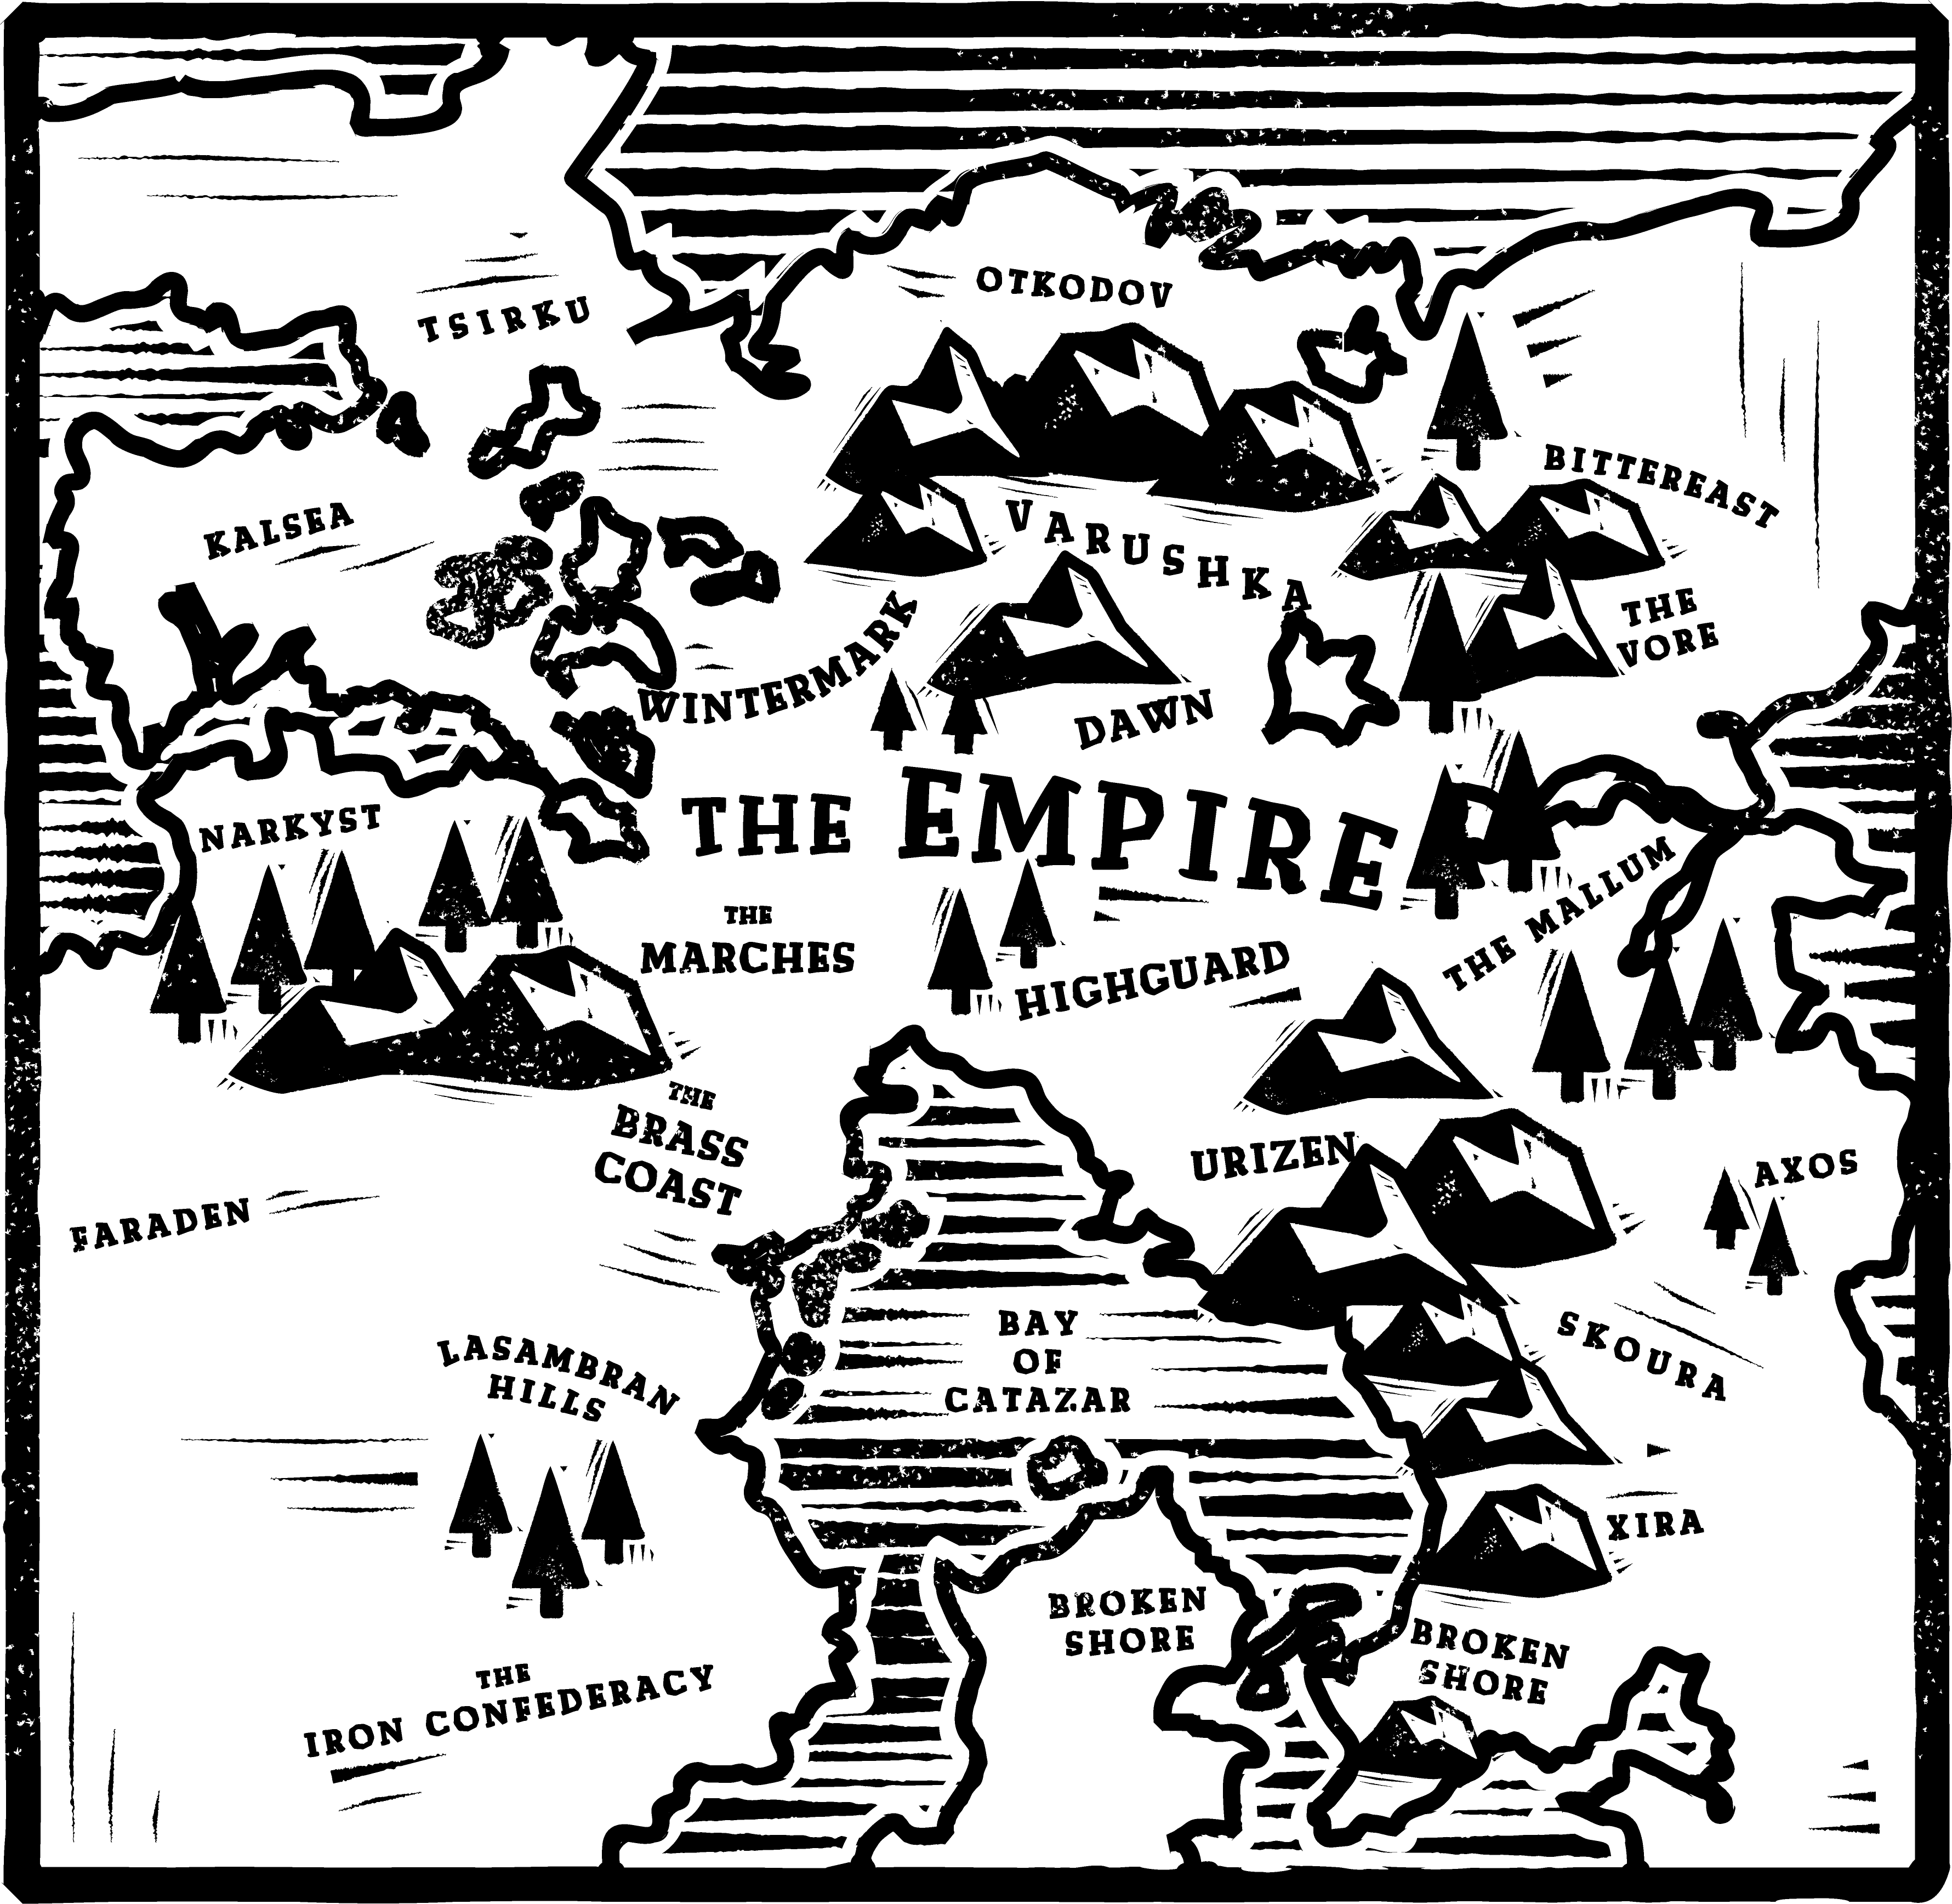
\includegraphics[width=0.9\textwidth]{encyclopedia/worldmap}\caption{the empire and its neighbours}\end{figure*}
\paragraph{freeborn} an inhabitant of the \see{brass coast}.
\paragraph{friar} a travelling monk
\paragraph{good walder} paragon of prosperity. Probably an early landskeeper.
\paragraph{green iron} a gray metal, generally symbolised by a sword. Used by magicksmiths to create dyes or lightwight \see{magickal item}s that offer protection.
\paragraph{hallow} a ceremony that gives a magickal item an aura of \see{virtue}, affecting everyone bound to the item.
\paragraph{hearth magick} is a low-key everyday type of magick that keeps us being safe and prosperous. It is also important for keeping the \see{Jack-in-chains} bound. Important elements of marcher hearth magick are the appropriate burial of marchers in marcher soil after \see{death} (cf. \see{holberg}), and many elements of tradition, such as \see{poppet}s and seasonal festivals, grant the marchers persistent prosperity through hearth magick.
\paragraph{hedges} a line of shrubs and important marker of the boundaries (\see{beater}) of fields and communities. As of new, it has become a tradition to bury dead \see{briar}s in the brambles of hedges.
\paragraph{herald}
\paragraph{herb} in addition to herbs useful in cookery and brewing, imperial herb gardens grow five herbs with important applications in \see{medicine}. \begin{table*} \begin{tabular}{p{0.6\textwidth}} blue mazzarine to save a limb\\ grey bladeroot stems a weakness dim\\ red roseweald venom’s power breaks\\ true vervain body's healing wakes\\ though marrowort takes soldiers' pain\\ at battle's end they'll fall again\\ \end{tabular}\caption{medical herbs}\end{table*}
\paragraph{herding cats}
\paragraph{heresy}the religious \see{crime} of willfully rejecting, or perverting, the orthodox doctrines of the faith as laid down by the imperial synod, or actively teaching and promoting false doctrines.
\paragraph{highguard} the \see{nation} that created the imperial \see{faith}.
\paragraph{holberg} the easternmost city of the league, notable for containing small enclave of marcher soil in \see{league}, where marchers were put to rest. The establishment was necessary because the bodies had been animated through a \see{winter} \see{ritual} to fight in the liberation of the city from the \see{druj}, which interfered with marcher \see{hearth magick} concerning \see{death} and awoke \see{Jack-in-chains}.
\paragraph{hunger} is a sign of lack of \see{prosperity}. Unfortunate marchers are welcome to help themselves to the fruits of the grave-orchards, and many places such as monasteries give support to increase the prosperity of downtrodden marcher folk. In anvil, hunger can be alleviated by dining at tyke’s.
\paragraph{husk} an animated corpse, eg. created by \see{winter} magick or \see{vallorn}. May need \see{burial} (cf. \see{holberg}).
\paragraph{idolatry}the religious \see{crime} of subsuming human will and destiny to any inhuman entity or force. This includes the worship, veneration or exaltation of any such being or power.
\paragraph{ilium} star metal, a valuable material with strong magickal properties. Ilium can make magick effects permanent.
\paragraph{injury} there are several different conditions afflicting the body to differentiate: a general loss in vitality; mortal wounds; terminal conditions; loss of limbs and some more special types of injuries. Other conditions, such as venoms or weakness, are discussed in the essay on \see{medicine}. Ways of restoring injuries are different for different injuries. A general loss in vitality can be restored through an apothecary using a dram of true vervain, …. When a yeoman has lost all their vitality and suffered a mortal wound, causing them to bleed out, they can be helped by …. An individual who has lost all their vitality and has lost too much blood to ever recover should have no hope return to this life, but …. Destroyed limbs can be restored through …. Other, more serious injuries and traumatic wounds need the attention of a skilled physick to be restored in a lengthy process, but a dram of marrowort can temporarily relieve the pain.
\paragraph{insight} a priestly ceremony that allows a monk to discern a mark on someone's soul.
\paragraph{iridescent gloaming} the wax from iridescent butterfly cocoons, generally symbolised by a butterfly. Used as colouring agent by magicksmiths who create \see{magickal item}s to enhance magick.
\paragraph{ISoM} the imperial school of \see{medicine}, founded upon marcher initiative, runs the anvil field hospital. Anyone with an eager interest in the medical arts of a chirurgeon, physick or apothecary will find much more intensive discussion of those matters in their wise library than in this loyal compendium.
\paragraph{Jack-in-chains} the dark mirror of the marcher egregore \see{Jack-in-the-green}. Same name as an evil giant from a children's story.
\paragraph{Jack-in-the-green} the marcher egregore. As every \see{nation} of the empire, all marchers are bound to an egregore. Jack is a \see{beater} and has been around for generations. The power of marcher \see{hearth magick} keeps his dark counterpart, the Jack-in-chains, bound deep in his core. If Jack-in-chains gets loose, he needs to be bound again by marchers following their traditions, and innocent \see{soul}s binding him in place, just like in the old legends we ken of the Jack-in-chains. The figures of Jack-in-the-green and Jack-in-chains may actually be older than the formation of the empire, for they have been part of legends even when the empire was founded.
\paragraph{joshua benson} exemplar of vigilance, recognized by the synod in 378. Known as “the major”.
\paragraph{jotun} the jotun are the tribe of barbarian orcs that have captured the \see{mournwold} in 347. They are a warlike tribe that values strength-in-arms and fighting-spirit as their highest virtues; they love one-on-one fights, challenged by the orc pointing at an opponent with their weapon and then raising their head up to show their necks to their opponent. Making a slashing or ripping gesture with their hand as they bring their head down with a snarl. This signal shows that they consider the person they are looking at as worthy of honourable combat. The target may return the challenge, and engage the jotun in single combat that ends until one warrior cannot continue. Jotun will usually accept a surrender unless they have reason to believe they are being tricked in some manner, and often allow injured opponents to retreat. They have also been kent to allow opponents who have fought bravely to gather their dead or injured. Warriors of the jotun see little honour in killing the weak or the unarmed, and prefer to take them as thralls. Thralls are treated reasonably well by the jotun; as long as they show proper respect to their overlords, they are usually left to their own devices. Many modern jotun thralls are the descendants of humans taken in battle, and consider the empire their enemy. The jotun value courage, strength and martial prowess above other attributes. Their love of battle and emphasis on personal glory and honour, as well as their war-like traditions, means that many jotun warriors are a match one-on-one for their imperial counterparts. They do not throw their lives away, nor use their subject tribes as disposable troops, but they are invariably looking for a way to increase their honour, with an eye towards becoming ancestors when they die. The only true dishonour most jotun recognise is showing fear in the face of the enemy, or striking a worthy opponent down by treacherous means. Jotun favour axes and hammers, both two-handed and coupled with a round shield. They tend to shy away from bows, and seem to have no appreciation for the crossbow as a weapon of war – when it comes to ranged combat they prefer thrown axes or javelins. The colour red appears to have totemic significance for the jotun, and figures on most of their banners. 
\paragraph{judgement} a decision of the \see{synod}
\paragraph{labyrinth}the twisting realm of pure spirit that is integral to the cycle of reincarnation, a core doctrine of the \see{faith}. The name is something of a metaphor for no mortal has been there to witness it, but the journey from death to rebirth is neither simple nor instantaneous. Some spirits are said to wander between lives generations before being reborn, and some are lost forever. The way of \see{virtue} teaches that living a virtuous life holds the key to successfully traversing the labyrinth of ages swiftly, safely and with the purity of spirit that strengthens ties to past lives.
\paragraph{law} marcher business is marcher business, and should be conducted as such. Tradition has means to settle \see{boundary dispute}s, \see{sorcerer}s, and so on. But when individuals from elsewhere are involved in an affair, the imperial code of law applies. This is often the case for events related to a summit in anvil. Under imperial law, \see{foreigner}s have the same protection as \see{citizen}s, though not the same rights. \see{barbarian}s do not have those rights, quite the opposite. Imperial law regulates crimes against people, crimes of position, crimes against the state, civil claims and religious crimes. The decision on guilt and punishment is made by a magistrate in a \see{trial}. The corresponding tables list all criminal acts; It is possible for willing participants to give consent so that what would otherwise be crimes being committed against them are not. Attempting, ading or abetting of a crime is equivalent to committing the crime under the law. \begin{table*}\begin{tabular}{p{0.15\textwidth}p{0.85\textwidth}} Murder& action against a person with intent to kill them.\\ Manslaughter& against a person which results in someone’s death.\\ Assault& striking a citizen. (Lack of lasting injuries can make fights legal.)\\ Mayhem& maiming or mutilating a citizen.\\ Poisoning& applying a poisonous substance or effect to a citizen which causes them harm.\\ Imprisonment& Unlawfully detaining a citizen against their will. Suspects must be directly supervised during any period of lawful custody.\\ Malsanguino& Willfully preventing someone from receiving medical attention with the intention of causing them harm.\\ Slavery& holding the power of life and liberty over any person, including \see{barbarian}s. \end{tabular}\caption{crimes against the person}\end{table*}\begin{table*}\begin{tabular}{p{0.25\textwidth}p{0.75\textwidth}}Theft& Dishonestly appropriating property belonging to another with the intention of permanently depriving the other of it.\\ Counterfeiting& falsifying, creating or amending of an imperial document or legal tender.\\ Criminal Damage& destroying or damaging any property either belonging to another citizen or to the Empire. \\ Breach of interdict & Owning forbidden items and substances. This includes drake's eggs, vallorn seeds, the Maggot's Talon wand, and the poisons gutwrench, moon's poison, hunger of the wolf, black gate and crimson gate. (for items interdicted by the conclave, the crime is against the processes of the state.)\\ Vallorn cultivation& Planting or tending vallorn is very likely to be interpreted to be vallorn cultivation, harvesting magickal ingredients from a naturally occurring vallorn pod may or may not be.\\ Trade of True Liao to foreigners& It is illegal to trade True Liao to anyone who is not a citizen.\\\multicolumn{2}{l}{\textit{Cases of negligence \&c. can be brought before forward in civil trials.}} \end{tabular}\caption{crimes against the person}\end{table*}\begin{table*}\begin{tabular}{p{0.25\textwidth}p{0.75\textwidth}}Treason& Aiding barbarians, eternals, or foreign powers to act against the interests of the Empire. Committing an assault against the emperor or empress. \textit{Only citizens and former citizens of the Empire may be charged with treason.}\\ Impersonation of an Imperial Official& Falsely and dishonestly claiming to be a senator, civil servant, member of the militia \&c., with intent to deceive.\\ Dereliction of Duty& Volunteering for an imperial duty and then failing to carry it out through neglect or cowardice. \textit{abuse of an imperial position is within the remit of the Synod.}\\ Vyig Membership & Membership in the criminal organisation, or possession of Vyig tattoos. \end{tabular}\caption{crimes of position}\end{table*}\begin{table*}\begin{tabular}{p{0.3\textwidth}p{0.7\textwidth}}Contempt of Court& any behaviour which impedes the proper operation of the legal process, such as disrupting a trial, or failing to attend court.\\ Perverting the Course of Justice& any behaviour calculated to unduly affect the course of the judicial process, such as bearing false witness, making false allegations, concealing offences or assisting others to evade arrest, interference with witnesses or evidence and evading, withholding or perverting a lawful punishment.\\ Subverting agencies of the state& any behaviour which contravenes or subverts the constitutionally protected procedures or powers of an agency of the state. \\ Resisting Arrest& Any course of action with the intent to oppose a lawful arrest.\\ Contravening a Declaration of Sorcery& as a declared sorcerer, owning crystal mana, performing rituals or interacting with Heralds and Eternals.\\ Improper placement of an aura on the senate building& The placing of an aura on the senate building without prior explicit permission from the Senate.\end{tabular}\caption{crimes against the processes of the state}\end{table*} \begin{table*}\begin{tabular}{p{0.2\textwidth}p{0.8\textwidth}}Idolatry& Subsuming human will and destiny to any inhuman entity or force. This includes the worship, veneration or exaltation of any such being or power.\\ Blasphemy&The denigration of the Paragons and the Paths of Virtue. This includes promoting False Virtues and the teachings, or example, of False Exemplars or False Paragons.\\ Heresy& The willful rejection, or perversion of, the Orthodox Doctrines of the Faith as laid down by the Imperial Synod, or actively teaching and promoting False Doctrines.\\ Abuse of Powers& The misuse, or abuse, of the powers of a priest. This includes the powers of the Synod, as well as liao ceremonies.\\ Desecration& The removal of spontaneously created auras such as legacies of ascendance to paragonhood. This includes such auras arising on areas, objects and people. \\ \multicolumn{2}{l}{\textit{Religious Crimes are tried by a magistrate but are raised by the Imperial Synod.}}\end{tabular}\caption{religious crimes}\end{table*}
\paragraph{league} a \see{nation} of city-dwellers, trying to turn \see{meade} into a city of their type. \see{holberg} is the easternmost city of the league.
\paragraph{liao} a refinement of vinum, used in priestly ceremonies. The very rare, pure liao allows citizens to experience visions of past lives.
\paragraph{lineaged} lineage means that a person is touched by one of the \see{magick}al realms and can occur in many ways. The table gives an overview of the types of lineage and their associated realms. Parents with lineage often give birth to children with their lineage, while the offspring of a human and a \see{herald} is always lineaged. It is also happens that fully human parents give birth to a lineaged child. Lineage can also occur for other reasons, for instance a child born in a primal forest under the influence of the realm of spring might become a \see{briar} in later life while a child born during a great famine when winter holds sway might be born a draughir. At certain times, the flow of magick due to constellation on the sky can influence the occurrence of lineaged, either naturally or by making transformative magick easier. Many marcher households are kent to not include any lineaged, despite appearance to the contrary – denying the merrow lineage of a household member by stating that he would be a mere human who is just feeling a bit blue –, or insist, for example, that their good cambions are spirited and energetic, whereas a cambion stranger would be seen as particularly conniving.\begin{table*}\begin{tabular}{lll} name& realm& trappings\\ \hline \see{briar}& spring& bark; volatile, impulsive \& restless behaviour\\ changeling& summer& pointy ears, antlers; bold \& self-confident attitude\\ cambion& autumn& curved horns; opinionated \& driven dominance\\ draughir& winter& pale skin, hollow eyes; cold \& hungry desire\\ merrow& day& gills, blue mottled skin; calm \& focused distance\\ naga& night& scales; relaxed \& passionate indulgence\end{tabular}\caption{the lineages}\end{table*}
\paragraph{loyalty} a \see{virtue}
\paragraph{magickal item} craftsmen can use the rare materials orichalchum (o), iridescent gloaming (ig), beggar’s lye (b) ambergelt (a), tempest jade (j) green iron (g), dragonbone (d), weltsilver (w) to create magickal items. Such items retain their special function for 4 seasons, after which they have to be re-charged, essentially creating the magick again from scratch. It does mostly take a magicksmith a full month to create an item; for such items as are empowered by skillful application of the artisan’s craftsmanship alone, and not through the magickal properties of their materials, it takes an artisan 2 full months. Personal magickal items can be armour, weapons or talismans (including shields). A magickian needs to create a bond between the bearer and the item, and every citizen can only have one bond of each of the three types. Magick jacks or mithril mail can still be worn under good steel. In addition, a group can have a magickal banner, covenstone or reliquary, and such item can aid every member of the group. The late pete keeper of king’s stoke has analysed and composed a selection of inexpensive, useful equipment for the soldiers of a marcher household, which is reproduced here for convenience. \begin{table*}\begin{tabular}{l}bolstering bill – a dying comrade may be saved once a day. 6 g, 7 w.\\ butcher’s bill – cleave a foe in twain or bowl them down once a day. 8 o, 2 ig\\ warden’s bardiche (bill) – another surge of heroic might. 10g 3 a\\ reaving mattock (great weapon) – shatter an armament once a day. 7j\\ oathkeeper’s bow – another surge of heroic might. 8 g 5 a\\ biting blade – this side-sword will cleave a foe mightily once a day. 7 o.\\ stoutheart gambeson (light jack) – an extra degree of fortitude, slowing the wearer’s bleeding. 2 months of a magicksmith’s time.\\ winter’s breath (light jack) – cure three of your wounds once per day. 5w 5a.\\ soldier’s harness (light jack) – the yeoman soldier may suffer another blow before she falls. 8a\\ mediator’s mail (medium weight) – cure three of your wounds with heroic might. 2 months of a magicksmith’s time.\\ mithril shirt (medium weight) – the yeoman soldier may suffer another blow before she falls. 2o 4a.\\ warrior’s plate (heavy steel) – the yeoman soldier may suffer another blow before she falls. 2 months of a magicksmith’s time.\\ phial of the sun – counts for the herb of a physick’s choosing, once per day. No use in potions. 3w 3 a 2 b.\\ chrysalis pendant – may use heroic might to set a broken limb. 8w 5a 3b. Expensive but valuable.\\ bannerman’s band: you may save a dying ally through heroic might. you may also do this for free once a day. 5g 4a 5d. Highly effective, more so than a bolstering bill. Lets you use your own reserves too.\\ pilgrim’s shield: the shield-bearer may suffer another blow before he falls. 2 months of a magicksmith’s time. User must be dedicated or anointed to a virtue.\\ alderman’s edge: a talisman allowing the wearer to use a bill, greatsword or spear with the ease of a weapons master. 8j 5d\\ bondring: you may bond to an ally as you would to a banner. you may heroically staunch their bleeding or cure a few wounds, once a day. 7d\\ wayfarer's pyx: when this reliquiary is \see{hallow}ed by a friar, the ceremony lasts as long as the item does. 2 months of a magicksmith’s time.\\ banner of the bold: all characters bonded to this banner are brave in the presence of even supernatural auras of fear. 2 months of a magicksmith’s time.\\ the effects of various covenstones are far too specific to be listed here.\end{tabular}\caption{the quartermaster's aide}\end{table*}\\
\paragraph{magick} mostly refers to what magickians do, but there is also \see{hearth magick}. Every magickian is able to perform three basic magickal effects. Magickians can create bonds between citizens and magickal items or groups (banners, covens or sects) of imperial citizens bound by a common oath. They can detect and to some extent identify magickal effects such as enchantments on items or individuals they consider, a ritual being cast in their presence, or magickal items. When considering a precise location at the sentinel gate, they can discern if there is a conjunction to that place; and if so, when it will open; how many people may pass through it; and any special circumstances that related to that conjunction. Finally any magickian can investigate and operate portals such as those bound to regios or the \see{sentinel gate}, including traveling through, allowing eternals to communicate through, or tracing where they recently opened to. While some magickians extend this number of spells by other useful incantations that mend equipment or problems of \see{medicine} or can be used offensively, many magickians focus on joining covens to cast \see{ritual}s, such as the mummery plays used to improve productivity of marcher farms. Rituals always correspond to one of the realms of magick, which are named (but at most metaphorically related to the seasons of) \see{winter}, \see{spring}, \see{summer}, \see{autumn}, \see{day} and \see{night}. An overview over rituals a landskeeper might come in contact with is given in an \see{appendix}. For a given problem, a vigilant landskeeper may be well served finding out which realm is likely to be relevant and find an expert on that realm for deeper wisdom.
\paragraph{magnitude} is a measure for the power of of a \see{magick}al ritual. Multiple landskeepers can cast a ritual together if they are in one \see{coven}, but a coven can only cast two rituals per day. [the magick maths: mastery, lore, regio]
\paragraph{major} (or mayor) 1. An old upwold word for steward 2. \see{joshua benson}, examplar of \see{vigilance}
\paragraph{mandowla} a legendary beast with a sturdy bear-like body with savage talons rather than claws and a head that resembles that of a giant owl with wide eyes and a savage beak. Often found in small family groups, they are omnivores – although with a marked preference for raw meat. They have a predator's cunning and are quite capable of attacking humans if they are disturbed or angered. They are most active at twilight, but have both excellent night vision and keen daylight sight. Common around upwold. These creatures are more dangerous than bears simply because they are so ready to attack and kill humans. They do not go out of their way to hunt humans, but if a family moves into an area containing a village, it will need to be dealt with. A small group especially one armed with long pole weapons should be able to bring one to bear and defeat it.
\paragraph{marches} a nation, bound to the egregore \see{jack-in-the-green}. \begin{figure*}\centering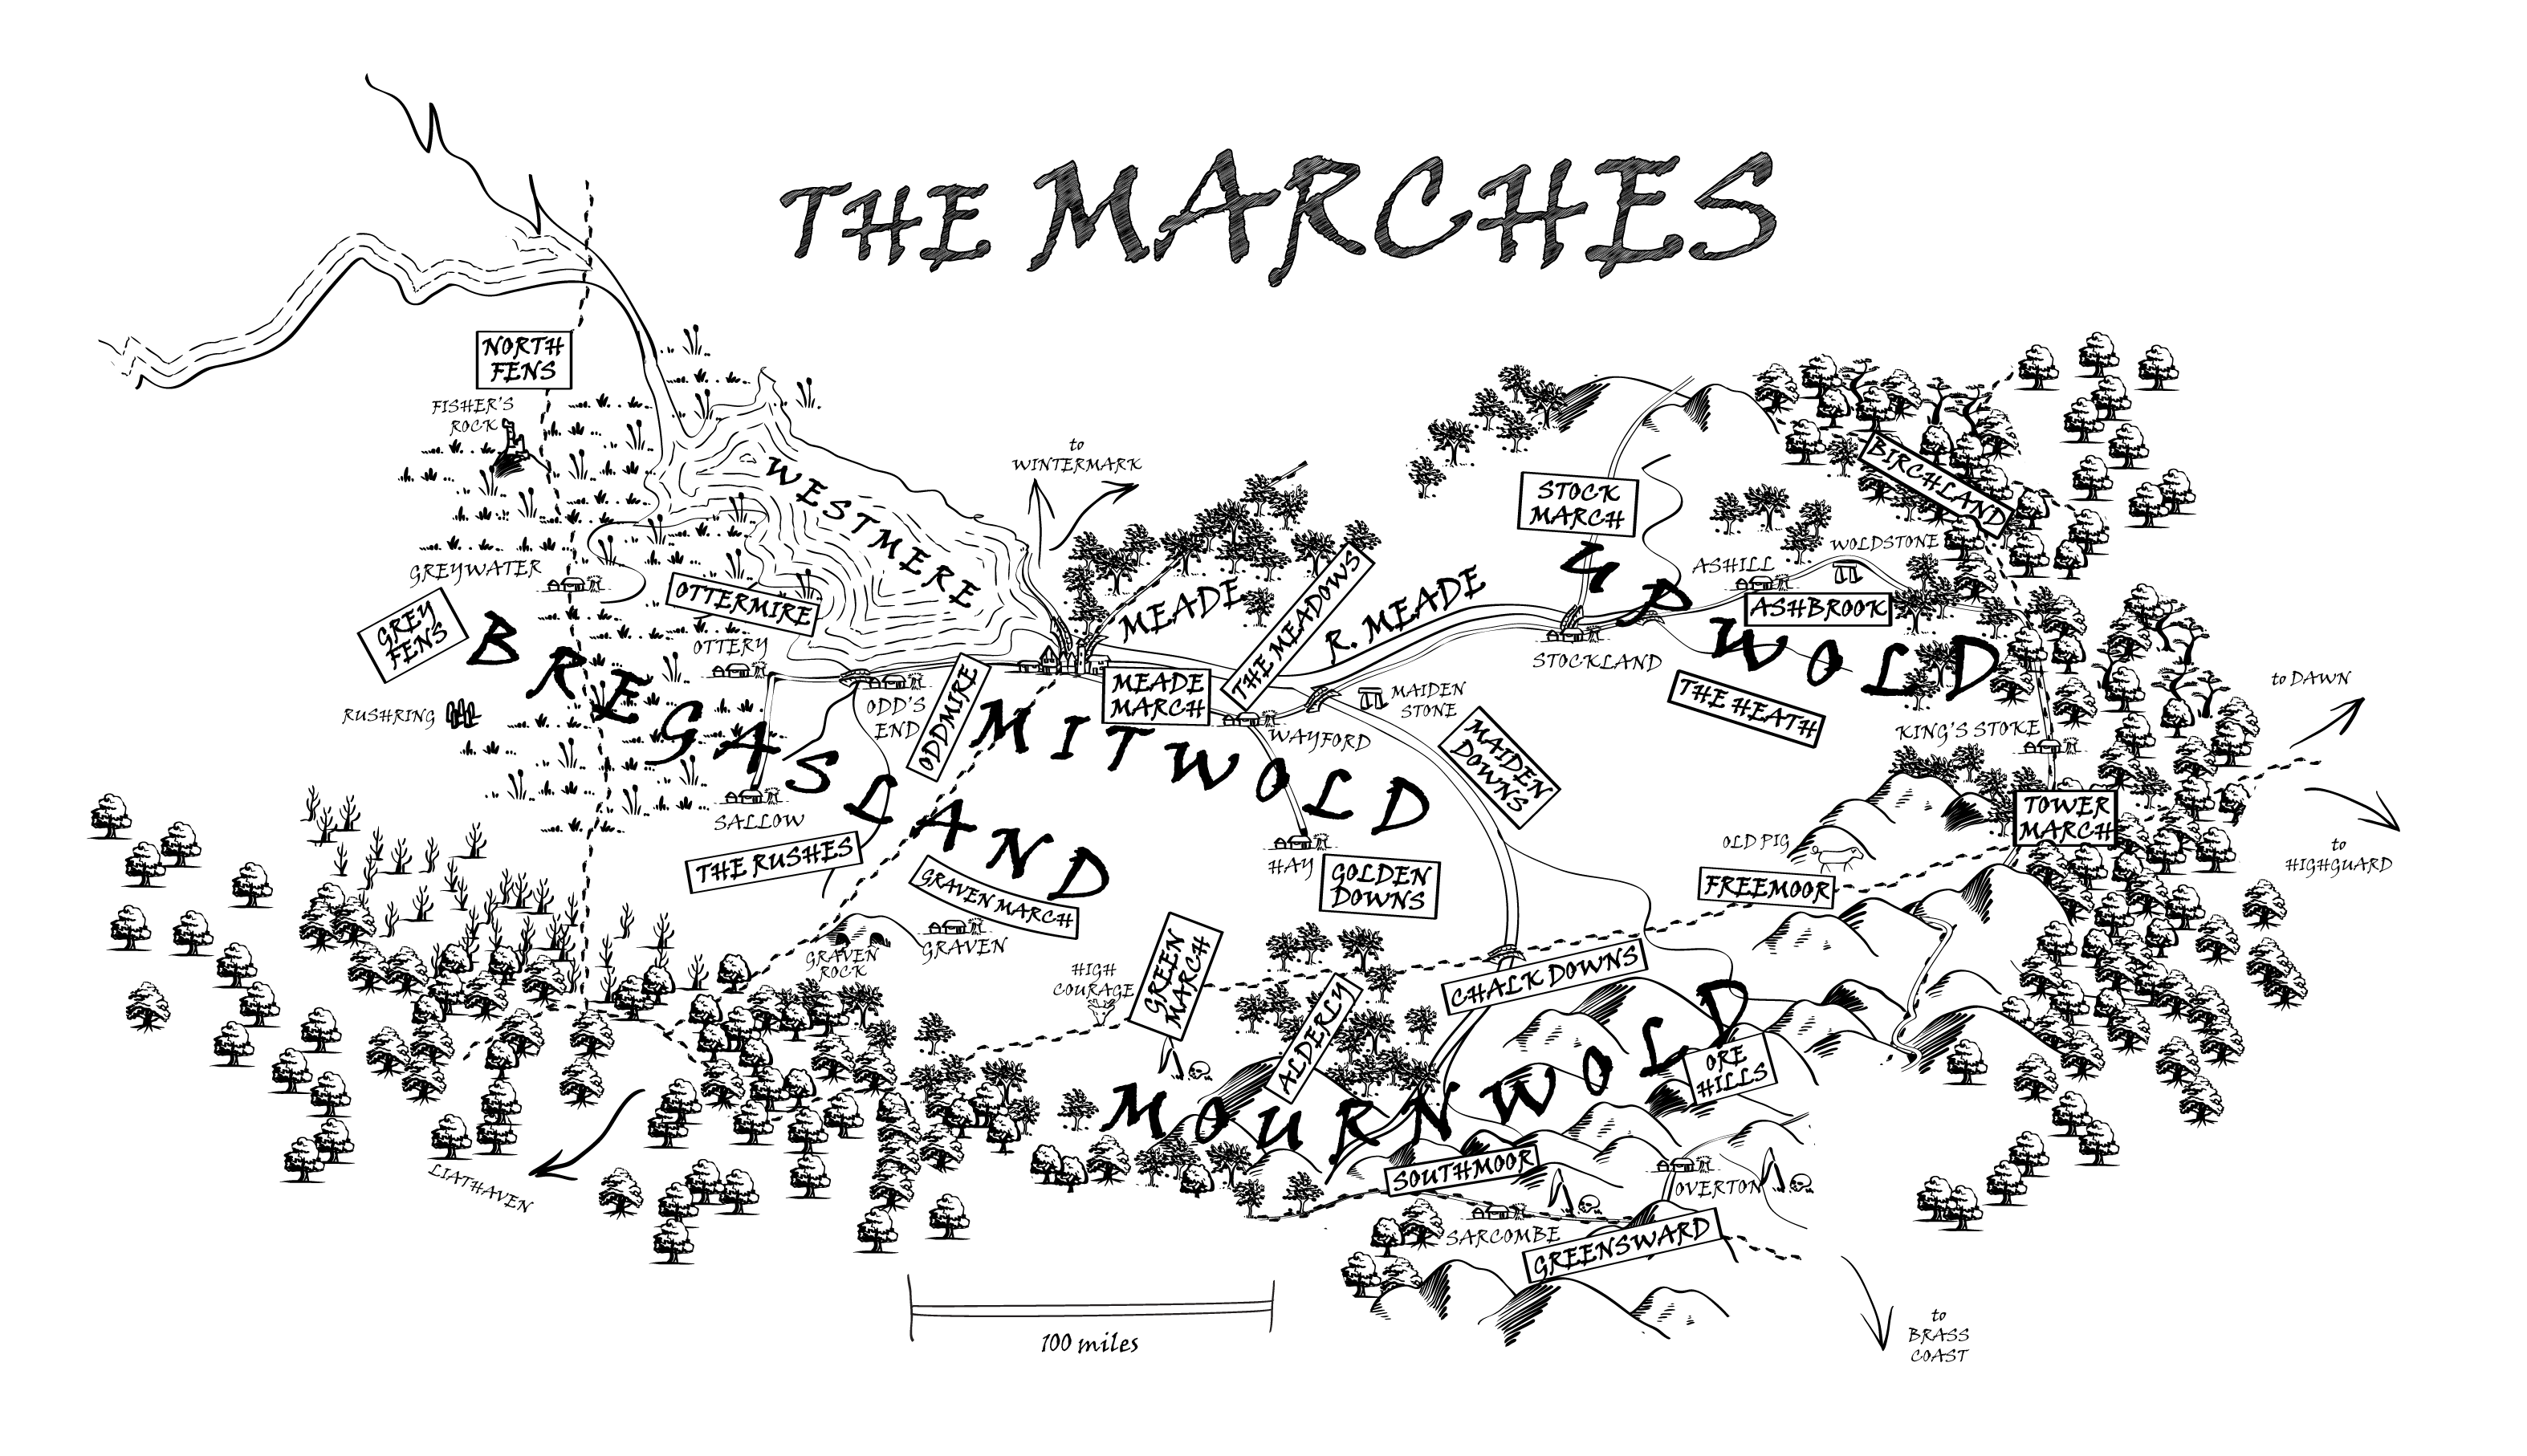
\includegraphics[width=1.1\textwidth]{encyclopedia/marches}\caption{the marches}\end{figure*}
\paragraph{march} the rebellion of marcher yeomen leaving dawn; transfered: becoming a marcher
\paragraph{marshwalker} a large semi-humanoid creature that appears to be made entirely of plant material, coated and held together with thick slime. Primarily found in marshy conditions, such as \see{bregasland}, the \see{druj} sometimes bring them along on battles. They are most dangerous when exposed to \see{vallorn}. One problem with marshwalkers is that, in their natural state, they are simply a colony of little slimy blobs that are virtually indistinguishable from the mud in which they live. In this state they are no threat to anyone, being primarily concerned with eating small insects, fish and plants and splitting into more tiny, nonthreatening blobs. It is only when they feel threatened, when some biological urge inside them decides it is time to move, or when someone starts building a structure near or threatening their habitat that the colony comes together to assume the much more dangerous form of a wood-armoured humanoid. Their migrations often take them near human settlements. Attempts to divert a marshwalker exodus are complicated by their resilience, their resistance to fire (they are simply too damp to burn), and their ability to smash through most obstacles placed in front of them. A marshwalker is a major threat to a village, and several marshwalkers might threaten a small town. A well-equipped militia can probably drive a marshwalker off, but are likely to take serious injuries in the process. A lone character can easily outpace one, and might be able to come up with a cunning way to divert one, but one-on-one will likely be quickly dispatched. 
\paragraph{materials} what a magicksmith uses to create \see{magickal item}s. \begin{table*}\begin{tabular}{lllp{0.5\textwidth}}name& shape&mark&effect\\\hline orichalcum&ingots of golden metal & shield& piercing; dissapating blows \\ tempest jade & chunks of green stone & lightning & decoration; polishing \\ green iron & ingots of gray metal & sword & lightweight protection; dyes \\ weltsilver & ingots of greenish metal & droplet & channeling energy; jewellery \\ ambergelt & chunks of red resin & wasp & healing, preservation; decoration \\ beggar's lye & bottles of tree ash & skull & caustic; changing material properties \\ dragonbone & sticks of marrow-clay & dragon & channelling bonds; clay-like shaping \\ iridescent gloaming & bottles of cocoon wax & butterfly & colour wash; enhancing magick \\ ilium & ingots of star metal & flame & making magick permanent \\ liao & bottles of liquid & labyrinth & priestly ceremonies \\ crystal mana & various crystals & certificate & casting rituals \\ \multicolumn{2}{l}{five imperial medical \see{herb}s} & certificate & \see{medicine}; \see{potion}s \end{tabular}\caption{trading commodities}\end{table*} \begin{figure}\centering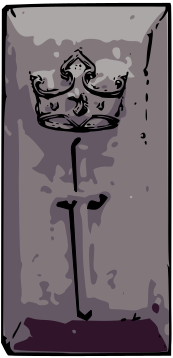
\includegraphics[width=2cm]{encyclopedia/greeniron} \quad 
\includegraphics[width=2cm]{encyclopedia/orichalcum}\caption{green iron (l), orichalcum (r)}\end{figure}
\paragraph{meade} a big market town in mitwold. Some misguided business owners from meade would like it to become a \see{league} city.
\paragraph{medicine} there are several afflictions of the body. In addition to \see{injury}, which is discussed in a separate section, age, venoms, weakness, and other effects can have an influence on a body. The \see{ISoM}, running the anvil field hospital, publishes more in-depths literature on medical matters. For the vigilant landskeeper, the conditions of venom and weakness and how to cure them will be most relevant. The most likely effect of a venom is to dilute the blood, speeding up bleeding and thus reducing the time in which a citizen with a mortal wound can still be saved. Such venoms can be cured by a physician using 1 dram of the \see{herb} imperial roseweald, by drinking a bloodhallow philtre \see{potion} (a red liquid with white particles), a magickian who has learned the purify spell, or a \see{day} ritualist using the \see{ritual} ascetic star of atun (m. 2); bearers of an abraxus stone or under the effect of the vitality of rushing water ritual are healed from venom whenever they are healed otherwise. Unnatural weakness can be removed by a physican using one dram of bladeroot, the feverfail elixir (a flowery, grey sirup), a magickian who has learned the purify spell, or a summer ritualist casting renewed strength of the new day (m. 2).
\paragraph{militia} thee militia are vital to the process of justice in anvil. They typically perform the bulk of any investigation work and brief the magistrates before cases go to \see{trial}. It is a constitutional obligation for a citizen who has been deputised into the militia to carry out their responsibilities. In practice it would only be in exceptional circumstances that a magistrate would suborn a citizen into the militia involuntarily. All serving members of the militia have the powers and obligations to take reasonable steps to prevent crime and maintain public order; to apprehend those suspected of crime(s) in progress and to bring them before a magistrate; and to report any crimes which require investigating to a magistrate. Magistrates will also appoint members of the militia to investigate specific crimes (a case). Members of the militia (and magistrates) may not enter a place of sanctuary without the express permission of a priest who is responsible for it. Even if permitted to enter they may not arrest or otherwise interfere with anyone within who has been granted sanctuary. An accused may only claim sanctuary for a limited period, usually one hour. This period allows the accused to make a confession and to ask a priest to attend them at trial so that a plea for clemency can be made on their behalf.
\paragraph{mitwold} the middle marcher territory, containing the large town \see{meade}.
\paragraph{monastery} a household of monks.
\paragraph{motion} a decision of the \see{senate}
\paragraph{mournwold} the southernmost marcher territory, lost to the \see{jotun}.
\paragraph{nation}one of the 10 composite people of the empire: the marches, \see{dawn}, the \see{league}, \see{varushka}, \see{wintermark}, \see{brass coast}, \see{urizen}, \see{navarr}, \see{highguard} and the imperial \see{orks}.
\paragraph{navarr} the \see{nation} treading the trods that reduce the \see{vallorn}'s power.
\paragraph{night} 1: a time 2: the \see{magick}al realm of passion, mystery and secrets
\paragraph{orichalcum} a golden metal, generally symbolised by a shield. Used by magicksmiths to create \see{magickal item}s that pierce or dissapate blows.
\paragraph{orks} 1. A species 2. The imperial orks, the \see{nation} encompassing all ork \see{citizen}s of the empire.
\paragraph{pilgrim} a \see{dedicate}d layperson
\paragraph{poison} a dangerous and illegal \see{potion}, such as gutwrench, moon's poison, hunger of the wolf, the black gate or the crimson gate.
\paragraph{poppet} every home in the marches has at least one straw dolly or poppet, made at the time of harvest to bring good luck to the house and ward off evil omens. These intricately twisted and knotted effigies of straw, corn, oats, rye, grass or rushes traditionally bind the vitality of the fields and bring their strength into the home. Many marchers carry their own small poppets for protection. In particular, every child is given a straw dolly of their own to help protect them from sickness, and an expectant mother will carry a poppet to ensure the health of the child. Touching someone else’s poppet can transfer good and bad between people, and should not be done. When the season turns again to sowing the seeds for the new crop these poppets are laid on the fields and ploughed back into the earth, or cast into a bonfire, ensuring a bountiful harvest for the following year. A landskeeper might employ a poppet in magick that binds or shares vitality or strength, such as granting potence of a band of yeomen. A \see{sorcerer} might use a poppet to steal the strength of an enemy or an enemy's fields, binding it as they twist and knot the doll until the poppet is destroyed or a year has passed. A friar might bind some of the \see{sin}s of a marcher to a poppet, to be taken away by the \see{wassail} fire, akin to a \see{wicker man}. To make a simple poppet, take a small bunch of stalks, around 8 inches in length, and strips of wool. Fold the stalks in the middle, and maybe bind them just below the fold and tie them tightly. Around a half inch to an inch below your first knot, do the same. Split the bundle into four strands, which will make the arms and body for your corn poppet. The middle two will become the body and the outer two strands will become the arms. Bend the stalks that make your corn poppet’s arms and bind carefully with the strip. Take a longer strip and tie it around the neck of your poppet. Bind the body pieces together and crisscross strips around the body. Take strips and tie them around the base of your corn poppet’s middle and body section. Split the bottom of your poppet to form the legs, just as you formed the arms, and bind them. For making a poppet from corn husks, see the figure.\begin{figure}\centering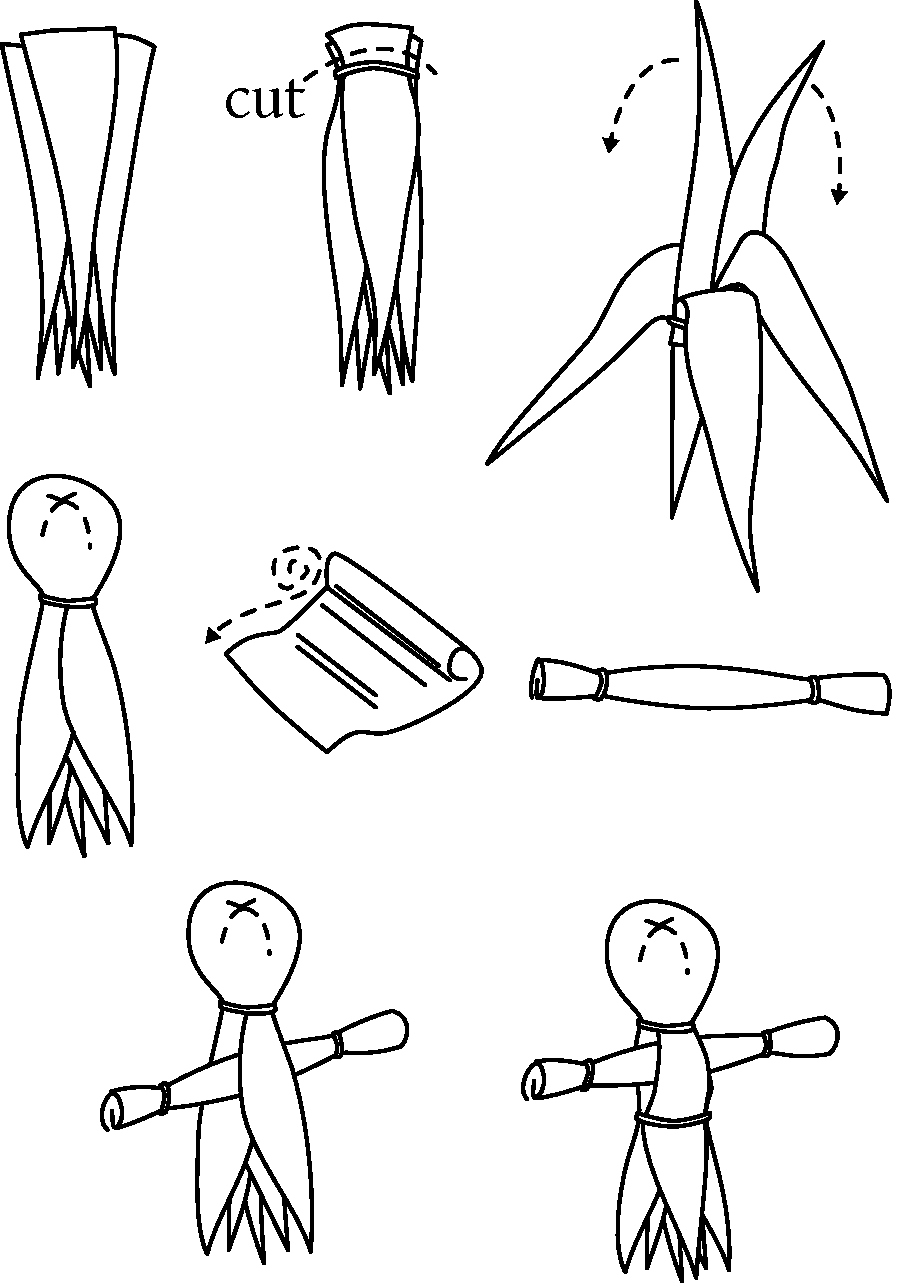
\includegraphics[width=5cm]{encyclopedia/poppet}\caption{making a poppet from corn husks*}\end{figure}
\paragraph{potion} brew of \see{herb}s with a supernatural effect. Every apothecary can create anodyne embrocation, bloodharrow philtre, elixir of life, feverfail elixir and ossean balm. For reference also listed are some other healing potions and poisons that need special attention. Some apothecaries can furthermore create potions that can influence citizens’ ability to perform rituals, religious ceremonies, heroic actions, \&c., but for those matters a vigilant landskeeper is better served finding a potions master or a tome on those items. \begin{table*}\begin{tabular}{p{0.15\textwidth}p{0.25\textwidth}p{0.35\textwidth}p{0.25\textwidth}} name &look &effect &ingredients \\\hline anodyne embrocation& numbing dark blue cream& temporarily numbs the pain from traumatic wounds& marrowort, true vervain\\ bloodharrow philtre& spicy translucent red liquid& body is purged of venom, and of some minor poisons& imperial roseweald, marrowort& elixir of life& sticky blue-green translucent liquid& heals loss of vitality& vervain, cerulean mazzarine& feverfail elixir& flowery grey sirup& cools the body and makes it regain strength& bladeroot, imperial roseweald& ossean balm& sandy blue salve& stabilises and heals a destroyed limb& cerulean mazzarine, bladeroot& gutwrench& viscous red-brown liquid& stomach feels on fire, possibly sweating, pain, weakness and venom& 2 imperial roseweald, 2 bladeroot, cerulean mazzarine& maledict's medicament& oily, deep crimson liquid & after some dizziness, quenches venoms out of the body and strengthens the body& cerulean mazzarine, bladeroot, imperial roseweald& tom drake's tea& viscous sweet-smelling yellow-green liquid& used to brew a pot of tea. Each person drinking a cup of the tea is fully revitalised after fifteen minutes of rest.& marrowort, bladeroot& philtre of strength& blue sweet, spicy smelling liquid. & regain a level of heroic might.& vervain, bladeroot.& oakenhide tonic& golden boozy liquid, tastes of apples.& take an extra blow before you fall. Gain confidence.& vervain, bladeroot.& sovereign specific& pleasant, tasty, sparkly clear liquid& thoroughly heals the drinker from all bad effects, including the pain from traumatic wounds& imperial roseweald, cerulean mazzarine, vervain, bladeroot marrowort. & moon’s poison& indistinguishable from water& a growing chill and numbing throughout all the body, reduced movement, coma, reanimation as a flesh-hungry zombie bent on killing and devouring the living. The wrong antidote speeds up the process.& 3 marrowort, 3 cerulean mazzarine, 2 vervain, 2 bladeroot.& hunger of the wolf& indistinguishable from water& a growing heat spreading through the body, extremely short temper, voices urging them to kill everyone around. The wrong antidote speeds up the process.& 4 imperial roseweald, 4 vervain, 2 bladeroot.& feast for the crows& lumpy red balm like rotting meat soaked in blood.& takes all vitality and delivers a fast death. The only antidote for hunger of the wolf and moonish slime.& 4 marrowort, 4 cerulean mazzarine, 3 bladeroot, 3 imperial roseweald, vervain. & the black gate& indistinguishable from water& dizziness, weakness, increased confusion, random pain, growing awareness of own death, hallucination of loved ones or dead relatives. \see{weakness}, agonising seizure, death. The wrong antidote speeds up the process.& 4 bladeroot, 3 vervain, 3 marrowort.& the crimson gate& indistinguishable from water& thirst, fever, agonising pain in joints and muscles, coughing blood, growing awareness of own death, venom. Blood from the eyes and nose, death through own blood. The wrong antidote speeds up the process.& 4 imperial roseweald, 3 vervain, 3 cerulean mazzarine.& the silver key& grey, resinous solution& uncontrollable cough, vomiting until stomach is empty. Loss of consciousness. Antidote to the assassin’s gate poisons.& 4 imperial roseweald, 4 bladeroot, 4 marrowort, 2 vervain, 1 cerulean mazzarine.\end{tabular}\caption{relevant potions}\end{table*}
\paragraph{pride} a \see{virtue}
\paragraph{prosperity} one of the seven \see{virtue}s.
\paragraph{proverbs} provide \see{wisdom} and guidance for all honest marchers. A collection of well-kent proverbs is included in the appropriate places in this book.
\paragraph{right of witness} synod priests are responsible for the spiritual wellbeing of the empire and are empowered to witness or observe all aspects of the bodies of state in function. In practical terms, it guarantees the right of synod priests to access the senate public gallery, even if the senate have called for a closed session and cleared citizens from the public gallery; observe the bourse private member's auction; be present in the military council tent during meetings of generals. (except senators, who are forbidden from entering or being present during the meetings of the military council); be present at a meeting of the conclave in the hall of worlds. The conclave has no responsibility for allowing non-magickian priests to reach the hall of worlds, and have repeatedly pointed out that a magickian who is a priest has every right to attend a conclave meeting anyway. The main use for the right of witness in the conclave is to observe the election of the grandmasters of the orders. Traditionally, the right of witness is also extended to the relevant bodies in the nations, such as the meetings of stewards, captains and landskeepers in the marches. Refusing a member of the synod the right to witness is a crime against the state under the \see{law}.
\paragraph{ritual} a powerful procedure creating a \see{magick}al effect, such as an \see{enchantment} or \see{curse}. Some relevant rituals are listed in an \see{appendix}.
\paragraph{rough music} making a loud noise around someone \see{sin}ful, such as a \see{sorcerer}, until they give up their leave or change.
\paragraph{scarecrow} a humanoid doll made from straw, wood and clothes. Scarecrows have a protective function according to \see{hearth magick}, similar to \see{poppets}.
\paragraph{senate} the primary legislative body for the empire, elected by the \see{citizen}s. In the marches, the steward who can unite the group of stewards and yeomen behind himself owning the most land gets to select the senator. Different stewards can oppose each other, even though they might nominate the same individual as senator.
\paragraph{sentinel gate} a \see{magick}al portal connected to the imperial regio in anvil. Every magickian has the skills to discern its conjunctions and operate it if a conjunction is happening.
\paragraph{shriven}\see{shriving}
\paragraph{shriving} the process of basic shriving is simple. A monk who is willing to take on a marcher’s faults or sins hears a confession. This can also be part of a preparation of a \see{clemency} plea in a trial, before the execution of a criminal, before a dangerous battle, or on the bedside of a marcher on the door to \see{death}. The confessor should confess freely and without restraint, when he is told that the monk is willing to shrive them. Whilst she listens, she weaves a poppet of straw, symbolically taking on part of his sin and embodying it in the poppet. Once he has finished his confession and the poppet is complete, she may offer a benediction of the way such as this: “may the way guide your footsteps on the earth, ambition grant you the will to strive, courage give you the strength to act, loyalty cleave you unto your fellows, pride inspire you to accept your past, prosperity let you feast on the fruits of your toil, vigilance keep you alert against falsehood, and wisdom keep you free of folly. May your sins be shared, your burdened halved, and your spirit guided by the virtues.” she may also spend the confessor an \see{anoint}ment. Once this is done, the shriving is completed, and the poppet should be burned at wassail along with offerings to atone unvirtuous deeds.
\paragraph{shunning} refusing to acknowledge the presence of an individual, ostracising them. Wicker men and such like must also be shunned.
\paragraph{sin} 
\paragraph{sorcerer} someone using magick for \see{sin}ful purposes. The \see{conclave} can declare someone a sorcerer, prohibiting them from magick under the \see{law}. \proverb{dark minds find dark places to do dark deeds}
\paragraph{soul} \see{virtue}s \see{doctrine}
\paragraph{sport and games} tug-of-war, foot-the-ball
\paragraph{spring} 1: a season 2: the \see{magick}al realm of the primeval force of life and growth.
\paragraph{steward} a yeoman leading a household
\paragraph{summer} 1: a season 2: the \see{magick}al realm of might and majesty
\paragraph{synod} the governing body for matters of \see{faith}, where all priests with a congregation have voting rights.
\paragraph{taint} a wild growth of dangerous supernatural and exotic plants where a \see{briar} was buried.
\paragraph{tempest jade} a green stone, generally symbolised by a bolt of lightning. Used for decoration and polishing by magicksmiths creating \see{magickal item}s. 
\paragraph{thule} the thule are inscrutable northern orcs, lead by \see{ritual}ists and fielding husks and fearsome beasts of war. Coming from the resource-poor north, they are stripping dead enemies, invaded regions and captured territories of anything valuable. Some of these resources are being used to reinforce their armies, but the lion's share is being sent north. Fighting against the thule is fierce, especially since the disastrous death of empress britta and most of her court. The thule favour dark, hooded robes and cloaks, emphasizing their size and bulk with fur pelts over their shoulders. Thule consider a dark blue hue to be fortunate and revere dragons and wyrms as totemic beasts full of potence and cunning.
\paragraph{traumatic wound} any extraordinary type of \see{injury} that is not just a general loss of vitality due to blows with weapons including mortal wounds, or loss of function of limbs. A physick will be able to diagnose and right traumatic wounds.
\paragraph{trial} trials settle disputes of law. They are presided over by a magistrate. It is their role to run trials in a manner which is expeditious and just. Magistrates will aim to conclude trials within ten minutes in most circumstances and so time given to both witnesses and the accused will be strictly controlled. The accused will be presented before the court. The accused may be accompanied by a priest (if they intend to plead guilty and ask for clemency) or possibly by a friend or legal advisor. The magistrate may choose to dismiss all the charges if they find no case to answer. Otherwise, the charges against the accused will be detailed and they will then be asked how they plead in relation to each charge: guilty or not guilty. If the accused pleads guilty then before pronouncing punishment the magistrate will allow any priest present (or the empress) to plead \see{clemency} on their behalf. Alternatively, if a weregild arrangement has been made with the victim then this must be approved by the magistrate. The magistrate may also investigate and consider any other pertinent evidence or testimony prior to sentencing. If the accused pleads not guilty then the magistrate will make arrangements for a trial to be held to investigate the facts of the case to determine guilt. If the accused refuses to plead then the magistrate may treat this as a guilty plea. In either case a plea for clemency will not be permitted. If all the relevant witnesses and evidence are available then the trial may proceed summarily. Alternatively, if further investigations are required or witnesses are not currently available, the magistrate will release the accused on their oath that they will present themselves when it is time for their trial. Occasionally a magistrate will set other limitations on the accused’s behaviour while awaiting trial. Where a magistrate has reason to believe that the accused is an absconsion risk or will not comply with their conditions they may require the payment of monies or assets to the court in surety. These assets will be returned after the trial, provided that the accused does not abscond, breach any conditions or commit any further crimes. If an accused absconds then the magistrate may try them in their absence. It is likely the magistrate will draw an adverse inference from the accused's failure to attend and also find them guilty of contempt of court. Any citizen can use reasonable force to apprehend them for the reward, although in practice it is often thief-takers and militia who are in the best position to do so. Exceptionally, the magistrate may order the accused to be held in supervised custody until their trial can begin. This is only permitted where the magistrate believes the accused would be likely to commit further crimes if they were released. If so, the trial must be carried out as soon as reasonably practicable. The magistrate is responsible for investigating the facts of the case, not for acting as an impartial referee. If the magistrate is satisfied that the accused is unable to represent themselves adequately for some extraordinary reason then they may allow another person to speak in their stead. This does not exempt the accused from the requirement to answer any questions put to them by the magistrate. Judgement is made by the presiding magistrate. Occasionally a magistrate may ask one or more of their peers to sit with them in judgement over a particularly difficult case. The law allows magistrates to accept any evidence, including hearsay. The minimum persons required to be present for a trial to be valid are the presiding magistrate, and at least one other person. The accused should also be present if possible, but may be tried in their absence if they abscond. Magistrates may choose to try all of those accused in connection with a particular crime or crimes at the same time. This is particularly likely where a criminal conspiracy by a group of individuals is suspected. Where there are multiple offences which might apply to the accused the magistrate is only required to set out the most serious charge(s). This does not prevent the accused from being found guilty of a lesser related offence. If found guilty, the punishment will also take into account any relevant lesser offences where appropriate. When determining the accused's punishment the magistrate will take into account the seriousness of the crime and any mitigating factors, for example presented by a priest in their plea for clemency.
\paragraph{trogoni} humanoid creatures with insect-like traits that live deep underground. They attack mana sites, consuming the mana crystals and feeding on the \see{magick}al flows. A single trogon is usually a match for an armoured warrior or two, with its tough carapace and savage rending claws.
\paragraph{upwold} the easternmost marcher territory, fortified.
\paragraph{urizen} a \see{nation} of kenning magickians.
\paragraph{vallorn} the vallorn appeard when terunael, an empire from \see{navarr}i prehistory, fell. From the hearts of their cities spread, a sick, infectious wave of life (\see{spring}) that crumbled stone, shot great trees up through streets and buildings, and warped what it found. Around the core of each city areas of spring appeared, resistant to all efforts to destroy them. These were named vallorn. Inside them are monstrous plants, the spores of which mutate living creatures that are exposed over many months. The air within the vallorn weakens those who enter, like venom. No complete catalogue exists – some things appear simply to be diseased, misshapen forest creatures, or mutated humans and orcs. Some seem to be plants, sporting a mass of tangled thorns or possessing abilities that make them dangerous to travellers. A common threat to those who venture into those areas where the vallorn is strong are the vallornspawn husks (animated corpses). That being said, there are non-vallorn spring monstrosities like marshwalkers or trogoni. It is important to remember that they behave basically like animals: show no fear, back off slowly and calmly, don't offer violence, don't block exits, don't bring yourself to their attention if you can help it, and \emph{do not play dead}. Climbing a tree may get you eaten by a tree.
\paragraph{varushka} a \see{nation} in the far north.
\paragraph{venom} many poisons (such as some \see{potion}s and the mists of the \see{druj} and \see{vallorn}) dilute the blood, making someone on the verge of death bleed out even faster. Ways of alleviating this are listed in the essay on \see{medicine}.
\paragraph{vermin} locusts: if you catch some of the locusts and burn them, the others will be stupefied by the smell: some will die, while others will fold their wings and wait to be caught, or will be killed by the sun. This arises from antipathy. Moreover, if you catch and burn a scorpion you will also catch the rest of the locusts, or drive them off. Weasels: they say that if one catches one of the weasels, cuts off its tail or testicles, and lets it go alive, one will not find any more of them afterwards on the same farm. House mice: house mice are killed if you put down black hellebore with barley meal. They will also run away from copper sulphate, and the seeds of oregano, celery and love-in-a-mist burned as incense. you can also employ such means as help against rats. Field mice: some farmers in mitwold have succeeded by blocking the holes with daffodils, so that as the field mice hurry to get out they will take the leaves with their teeth. When they bite them they will die. Foxes: a fox will not bite any bird under whose wing you have fastened wild rue. Snakes: no snakes will enter the farm if you plant wormwood or mugwort or southernwood around the farmstead; you will drive away those that are already there if you make smoke with white lily root or stag’s horn or goat’s hoof. Snakes will not trouble the pigeon-house if in its four corners you write adam: if it has windows, write it at these too. When a snake is going into its hole, if one catches its tail with the left hand one will easily pull it out again; if with the right hand it will be impossible to get it out. Either it will escape, or the tail will break off. Scorpions: if you rub your hands with radish juice, you can pick up scorpions and other such creatures without fear and without danger; and radishes, placed on scorpions, destroy them immediately. By frying a scorpion in olive oil and consecrating the place where someone has been stung by a scorpion you will alleviate the pain. Ants: if you catch and burn some ants you will drive away the rest of them, as experience has proved. If you spread cedar oil around their holes, ants will not come on the threshing floor. Ants will not attack a heap of grain if you draw round the heap with white earth, or put wild oregano around it. Mosquitoes: horsehair stretched across the door and through the interior of the house destroys mosquitoes and prevents them from entering. If you soak a sponge in sharp vinegar and hang it at your head and at your feet when in bed, the mosquitoes will not bite you. Bats: if you hang plane leaves in their path, they will not approach. Smoked ivy kills bats. Fleas: in the house, dig a hole; grind oleander leaves and place in it; they will all gather there. Otherwise, soak the floor repeatedly with amorge; then grind wild cumin and mix with waters, and grind 10 drams of squirting cucumber seed and add to the water; sprinkle this in the room and you will make the fleas split. Leeches: if an ox or other quadruped swallows a leech while drinking, squash some bugs, let the animal smell them and it will immediately eject the leech. Frogs: frogs will stop their croaking if you light a candle and put it on the river-bank. Rats: rats reproduce quicker than any other animal, and harm your corn, bacon, cheese and other provisions. Fortunately, the natural enemies of rodents can be employed, by having a good array of cats. A cat corpse with a dead mouse stuffed in their mouth is sometimes built into the foundations of a house as it deters other rodents from entering the premises. To catch rats, rat-catchers employ traps made of little planks upon sticks or poisoned bait of an ounce of aconite, two ounces of fine arsenic, a quarter of pig's fat, a pound of fine wheaten meal and four eggs, made into a bread and cooked in the oven and cut into strips; or cakes of paste and powdered aconite, setting these near to their holes where they have naught to drink; or black hellebore mixed with fat, bread, cheese or flour; or the juice of bruised wild cucumber, which slays the mice as diverse men have said.
\paragraph{vigilance} a \see{virtue}
\paragraph{virtue} the \see{faith} of the way is composed of the seven virtues \see{loyalty}, \see{vigilance}, \see{ambition}, \see{courage}, \see{pride}, \see{wisdom}, and \see{prosperity}, and imperial priests can perform ceremonies that actualise these virtues in the world. Individuals following the virtues transit through the \see{labyrinth} faster and can ultimately leave it behind and become paragons. False virtues, such as hope, \see{fear} or peace, try to steer honest \see{citizen}s away from the way.
\paragraph{wassail} after every harvest, marcher farmers perform this traditional religious ceremony to celebrate prosperity. Wassailing varies from place to place but typically involves parading through the village singing and drinking to the health of the fields and orchards. Food and drink produced during the year is consumed or left as an offering; ale might be used to toast a barley field or a pat of butter buried in a dairy pasture. The parade is often led by the children of the village. As the yeomen go from house to house they share food and drink with their community and receive in return a taste of the food that each household has in excess from their own harvests. At each autumn equinox, marchers parade from camp to camp, singing the wassail and sharing their home-grown produce with other nations. Although not expected, other nations often reciprocate in small token exchanges of goods that their own territories have in abundance.
\paragraph{weakness}\see{medicine} a medical affliction of the body
\paragraph{weltsilver} a slightly tinted silver metal, generally symbolised by a blood droplet. Used by magicksmiths to create jewellery or \see{magickal item}s that channel energy.\begin{figure}\centering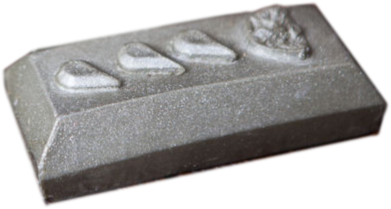
\includegraphics[width=4cm]{encyclopedia/weltsilver}\caption{weltsilver}\end{figure} 
\paragraph{wicker man} this is a large figure of wicker and wood, which is set alight to burn sacrifices at \see{wassail}. Ideal sacrifices are things that have been raised by mortal hands from the land such as crops and domesticated animals. These sacrifices are made to atone for \see{sin}s. By giving up the rewards of \see{prosperity}, and creating the need for more prosperity to replace them, the marchers believe that they make reparation for their unvirtuous behaviour and in this way ensure that they reincarnate well in the next life. The greatest sacrifice of all is to give up ones own life. This is only ever permitted for individuals whose failure cannot otherwise be redeemed. By going voluntarily to the wickerman they absolve not just their own failure but the failures of everyone who served under them. The most recent example was in 349 when former senator thomas overton of the mournwold went into the wicker man to absolve himself for his inability to keep his territory out of jotun hands. Similarly to the wicker man, many marchers burn their poppets at wassail to atone for small \see{sin}s and transgessions. 
\paragraph{wintermark} a \see{nation} of there different people north of the marches.
\paragraph{winter} 1: a season 2: the \see{magick}al realm of cruelty and choices
\paragraph{wisdom} a \see{virtue}
\paragraph{yeoman} a farmer who owns the land they toil

\chapter{some useful rituals}
\label{appendix}
while imperial lore contains a great number of different rituals in all the different realms, even a landskeeper not practicing the magickal arts themself should be aware of some useful rituals, and at least roughly ken what is necessary to enact them.
\paragraph{strong ox, golden sun} summer \see{magnitude} 4. This ritual targets a farm which must already be enchanted with the blessing of new spring ritual. The character who controls the target personal resource must be present throughout. This ritual completely replaces the effect of blessing of new spring. The target farm earns an additional 50 rings at the summer solstice (event 3) and the autumn equinox (event 4). The ritual ends at the start of winter. This spell is intended to be cast at the spring equinox. If the spell is cast later in the year, then money that would have been gained in earlier seasons is lost. It is useless if performed after the summer solstice. This ritual can affect additional farms in the same territory. Each additional farm increases the magnitude by 2.
\paragraph{blessing of new spring} spring \see{magnitude} 2 this ritual targets a farm. The character who controls the target personal resource must be present throughout. This spell is an enchantment. A target may only be under one enchantment effect at a time. The farm earns an additional 10 rings at the spring equinox (event 2), the summer solstice (event 3) and the autumn equinox (event 4). The ritual ends at the start of winter. This spell is intended to be cast at the winter solstice. If the spell is cast later in the year, then money that would have been gained in earlier seasons is lost. It is useless if performed after the summer solstice. This ritual can affect additional farms in the same territory. Each additional farm increases the magnitude by 1.
\paragraph{gathering the harvest} autumn \see{magnitude} 15. This ritual targets a farm which must already be enchanted with the strong ox, golden sun ritual. The character who controls the target personal resource must be present throughout. This ritual completely replaces the effect of strong ox, golden sun. The farm earns an additional 400 rings at the autumn equinox (event 4). The ritual ends at the start of winter. This spell is intended to be cast at the summer solstice. If the spell is cast earlier in the year, then money that would have been gained from strong ox, golden sun or blessing of new spring is lost. The effect lasts until the start of the next profound decisions empire event. If the owner of the resource does not attend the next event, then the additional production provided by the resource is still added to that character's inventory. This ritual can affect additional farms in the same territory. Each additional farm increases the magnitude by 12.
\paragraph{bright lantern of ophis} day \see{magnitude} 6 the ritual reveals information about an enchantment, \see{curse} or other magickal effect. It is most often used on a character or item that is present. It can also be used on a special effect that is anchored to an area. It determines the realm and magnitude of the effect; it determines what the effect does, and provides details of how it works; it reveals any remaining duration; it reveals any conditional effects, or any special methods that exist for removing the effect; it may provide information about where the magickal effect has come from (a ritual or the supernatural abilities of an eternal, for example). you may increase the magnitude of the ritual to penetrate more powerful shrouds or masks.
\paragraph{circle of gold} autumn \see{magnitude} 9 this ritual targets up to five characters from the same band. Each character must be present throughout. The target characters gain the ability to use stay with me once without needing to ken the skill or spend any hero points; however, they can only use the ability on another character who was also a target of this ritual. They feel a desire to stick together, whether on the battlefield or off it. They feel a strong urge to defend the other targets of the ritual, whether from physical harm or from insults. The effect lasts until the end of the next battle, skirmish or quest the character participates in; or until the end of the current event, whichever is sooner. This ritual can affect additional characters from the same band. Every two additional characters increases the magnitude by 3. Additional characters must be present throughout. Any caster who has mastered the ritual may choose to substitute weltsilver for crystal mana when contributing to it. Every 2 ingots of weltsilver spent counts as 1 crystal mana when contributing to the ritual.
\end{document}
